\chapter{模态逻辑,知识逻辑}\label{chap:modal-logic}

你听说过魔芋与高僧的故事吗?相传,这个有趣的故事发生在日本的一座深山之中. 在那幽静的山谷中,有一座古老而荒废的寺庙,几百年来一直无人问津,只有密林与野兽相伴. 

一天,一个以卖魔芋为生的流浪小贩推着他的木车,偶然来到这片偏僻的地方. 他发现这座破旧的寺庙中竟然无人居住,便心想:“如此偏僻之地,不如就在此安顿下来吧. ”于是,他便住了下来,每天挑着魔芋,走村串户,卖给山中偶尔路过的行人. 

不久之后,一位云游四方的僧人也来到了这片深山. 看到这座荒废的寺庙,他心生好奇,便前去查看. 僧人惊讶地发现寺庙中竟然住着一位老人,便以为这是位得道高僧. 僧人心中一动,想着既然能在如此偏远之地修行,必定有过人之处,于是便恭敬地上前,请教佛法. 

在佛教传统中,有一种不动声色的辩经方式,那就是只用手势来比划,而不发一言. 僧人遵循这一传统,开始用手势向卖魔芋的人比划起来. 然而,卖魔芋的人哪里知道这些佛教传统?他误以为僧人是在挑剔他卖的魔芋不好,来讨说法的. 他心中不悦,但还是用手势回应僧人,心想着:“我卖的魔芋可是顶好的,若是敢挑衅,我便和你理论理论!”

于是,两人各怀心事,展开了一场激烈的手势比划. 僧人暗自佩服卖魔芋的人的沉稳与深不可测的手势,心想自己在佛法修行上还有很大的差距;而卖魔芋的人则越比越得意,心中大呼:“这人还真有些手段,但我魔芋的品质岂是一般人能质疑的?”

比划结束后,僧人心生敬意,深感不如;卖魔芋的人则自信满满,觉得自己的魔芋赢得了这场对峙. 因此,“卖魔芋的人获胜”这件事成了他们二人的共同知识. 然而,两人心中所思所想却完全不同!僧人认为自己遇到了高人,而卖魔芋的人则确信自己击退了一个挑刺的顾客. 

在\Cref{chap:bayesian-game}中,我们探讨了知识的一些基本性质. 上面的魔芋故事实际上揭示了两件重要的事情:
\begin{itemize}
    \item 一方面,知识(尤其是共同知识)要比我们想象的复杂得多. 在这个例子中,两个人知道的“事实”究竟是不是同样的呢?这个问题并不容易回答. 
    \item 另一方面,知识的传递与理解可以超越自然语言. 在这个例子中,两人完全没有用语言交流,而是依靠手势. 这说明知识可以有不同于自然语言的表达方式. 
\end{itemize}

在本章中,第二点将是我们的讨论重点. 它意味着我们可以用形式逻辑来描述知识的概念和性质. 这种形式逻辑在现代逻辑学中被归类为\textit{模态逻辑}. 模态逻辑是一种扩展了经典形式逻辑(如命题逻辑和一阶逻辑)的逻辑,通过引入\textit{模态词}——例如“必然”、“可能”、“知道”等——来描述命题的性质. 最后,作为一个例子,我们将使用模态逻辑的语言表述并证明Aumann的“对不一致达成一致”定理. 

\section{知识逻辑的形式语言}

\textit{模态词}是指说话者对语句的限定. 不同的限定反映了不同的逻辑状态. 例如:\textit{必然}、\textit{可能}、\textit{过去}、\textit{未来}、\textit{知识}、\textit{信念}和\textit{可证明}等,都是典型的模态概念. 比如,我们可以说“明天可能会下雨”、“我知道明天会下雨”、“我相信明天会下雨”、“明天可能会下雨”等等,他们要表达的意思并不是经典逻辑可以表述的. 

在经典逻辑中,我们只能表达“明天下雨”或者“明天不下雨”这样的命题. 因而,\textit{模态逻辑}提供了一套严密的数学工具,可以把模态的概念从自然语言中“搬到”形式语言中. 

因为模态词往往都与人的认知和思维有关,因此,通过模态逻辑,我们可以算法化、自动化地模拟和推理人类的思维和认知过程. 这正是人工智能中\textit{符号主义}的思想. 

在研究模态逻辑时,重要的一部分是研究它的\textit{模型论},即如何定义模态逻辑的语言、然后赋予这些形式语言具体的含义与真假,即\textit{语义}. 

模型论的角度看,一个逻辑系统包括三个要素:\textit{语言}、\textit{模型}、\textit{语义}. 他们分别代表,我怎么说话、我关心的对象是什么、我说的话和我关心的东西之间有什么关系. 接下来,我们以命题逻辑为例,介绍三要素. 

\begin{example}[命题逻辑的逻辑三要素]
命题逻辑是由命题字母、逻辑联结词和括号组成的形式语言. 例如,$p\to q$这样的东西属于命题逻辑,但是$\forall x\, P(x)$这样的东西不属于命题逻辑(而属于一阶逻辑). 关于命题逻辑更系统的讨论,请参阅\Cref{chap:plausible-reasoning}. 

命题逻辑的三要素是:

\begin{itemize}
    \item 语言(我怎么说话):用规则写成的字符串,例如我们可以用字符串$p\to q$表示一个逻辑公式,但是不能写$\forall x\, P(x)$、$2+2=4$或者$p\vee\vee q$. 我们可以简单理解成,我们说普通话的时候,不能说英语,也不能说语法错误的句子(如“我是是”). 
    \item 模型(我们关心的对象是什么):我们关心的世界结构,在命题逻辑中就是“真”和“假”. 因此,在命题逻辑的世界里,没有实数,也没有人类,更没有诗和远方;只有冰冷(但是精确)的“真”和“假”. 
    \item 语义(我说的话和我关心的东西之间有什么关系):我们可以先给命题字母真假的概念,例如$p$赋值为“真”,$q$赋值为“假”. 当每一个命题字母都被赋予了真假之后,我们就可以定义整个公式的真假. 例如,$p\to q$为真当且仅当$p$为假或者$q$为真. 
\end{itemize}
\end{example}

尽管在\Cref{chap:plausible-reasoning}中,我们也简要介绍了逻辑三要素. 但是,我们在这里才将这样的讨论展开. 这是因为,只有到了模态逻辑的世界,逻辑三要素才变得如此不平凡,我们才能真正体会到他们的意义. 接下来,我们将介绍模态逻辑的语言、模型和语义. 本节先介绍模态逻辑的语言. 

首先,我们只考虑最简单的情况,基础语言是命题逻辑,然后在其中加入一个\textit{模态算子}. 

\begin{definition}[基本模态语言]
给定命题字母表$\mathbf P$,我们定义它的\textbf{基本模态语言} $L$,按照如下方式递归生成:
\begin{itemize}
    \item 命题字母$p\in \mathbf P$属于$L$,$\top$属于$L$. 
    \item 如果$\phi$属于$L$,那么$\neg\phi$ 和$\Box\phi$也属于$L$. 
    \item 如果$\phi_1,\phi_2$属于$L$,那么$(\phi_1\wedge\phi_2)$也属于$L$. 
\end{itemize}
\end{definition}

和命题逻辑比较,我们多了一个模态算子$\Box$,它读作“Box”,对应的自然语言可以读为“必然”(更多讨论见本部分后文). 

我们在后面将会频繁定义各种不同的模态语言,为了方便,我们引入一种更简洁的记号:
\[\phi\quad::=\quad p\mid \top\mid \neg\phi\mid (\phi\wedge\phi)\mid \Box\phi.\]
这种记号被称为\textit{Backus-Naur范式}(\textit{BNF}),是一种用来描述形式语言的标准记号,在编程语言设计和编译器的实现中也经常使用. 

类似命题逻辑,我们有如下缩写:
\begin{itemize}
    \item $\phi\vee\psi\iff\neg(\neg \phi\wedge\neg\psi)$.
    \item $\phi\to\psi\iff\neg\phi\vee\psi$.
    \item $\bot\iff\neg\top$.
\end{itemize}

引入模态算子$\Box$之后,我们还有它对应的\textit{对偶}算子$\Diamond$,它是如下的缩写:
\[\Diamond\phi\iff\neg\Box\neg\phi.\]
$\Diamond$读作“diamond”,对应的自然语言可以读为“可能”. 为什么它的自然语言解释是“可能”呢?因为,“不是必然不”的意思就是“可能”. $\Box$和$\Diamond$的对偶性,我们可以类比$\exists$和$\forall$的对偶性,这是因为$\exists$也可以写成$\neg\forall\neg$. 我们将在\Cref{sec:kripke-semantics}中看到,这一类比其实有极其自然的模型论解释. 

既然可以加入一个模态算子,我们也可以加入更多的模态算子,一个模态算子也可以修饰多个公式. 例如,我们可以引入一个新的模态算子$\Box_a$,表示个体$a$认为的必然性. 于是,我们可以写出这样的公式:
\[\Box_a\phi\wedge\Box_b\psi\to\Box_a(\phi\wedge\psi).\]
我们也可以引入模态算子$\nabla(\phi,\psi)$,表示$\phi$成立的时候,$\psi$必然成立. 于是,我们可以写出这样的公式:
\[\nabla(\phi\to\psi,\Box\phi)\to\Box\psi.\]

通过引入不同的模态算子来描述不同的对象,模态逻辑被赋予了这样的哲学:多视角下看同一个数学概念. 比如,我们可以把$\Box$在自然语言中用不同的词来解释,由此得到不同的模态逻辑:
\begin{itemize}
    \item 基本模态逻辑:可能/必然是
    \item 时序逻辑:将会是
    \item 道义逻辑:被允许是
    \item 知识逻辑:被知道是
    \item 可证性逻辑:可以被证明是
    \item 动态逻辑:(在经过某些程序步骤之后)会是
\end{itemize}

接下来,我们具体看两个例子,这是本节最关心的两种解释:\textit{基本模态逻辑}和\textit{知识逻辑}. 
\begin{example}[基本模态逻辑]
我们可以把模态算子$\Box$读成“必然”. 于是,
\begin{itemize}
    \item $\Box\phi$ 表示“必然有$\phi$”. 
    \item $\Diamond\phi$ 表示“不是必然有非$\phi$”,即“可能有$\phi$”,所以$\Diamond$读作“可能”. 
    \item 反之,$\Box\phi$也可以读作“不可能有非$\phi$”,即“必然有$\phi$”. 
    \item 因此,$\Diamond$和$\Box$确实是对偶的. 
\end{itemize}

在这个读法下,我们可以用形式语言去表达一些自然语言中很拗口的句子,但更加清晰和精确. 比如:
\begin{itemize}
    \item $\Box p\to\Diamond p$:必然的事也是可能的. 
    \item $p\to\Box p$:真的事是必然的. 
    \item $\Diamond p\to\Box\Diamond p$:可能的事是必然可能的. 
\end{itemize}
\end{example}

\begin{example}[知识逻辑]

在知识逻辑中,我们可以把模态算子$\Box$读成“知道”,并写成$K$(know). $K$表示某个特定的个体对世界的认知. 例如:

\begin{itemize}
    \item $K\phi$(即$\Box\phi$):我知道$\phi$. 
    \item $K\phi\to\phi$:如果我知道$\phi$,那么$\phi$是真的. 
    \item $\phi\to K\phi$:如果$\phi$是真的,那么我知道$\phi$. 
    \item $\neg K\phi$ vs. $K(\neg\phi)$:我不知道上帝存在 vs. 我知道上帝不存在. 这两句话的含义是不同的,因此,模态词使得否定的含义变得复杂. 
\end{itemize}

在更一般的情况下,我们会有多个个体,于是可以用$K_a$表示“个体$a$知道”. 同样,我们可以用$B_a$表示“个体$a$相信”. 这里是一些例子:

\begin{itemize}
    \item $K_aK_b\phi\leftrightarrow K_bK_a\phi$:我知道你知道$\phi$当且仅当你知道我知道$\phi$. 
    \item $K_1K_2p\wedge \neg K_2K_1K_2 p$:$1$知道$2$知道$p$,但是$2$并不知道$1$知道$2$知道$p$. 
    \item $\neg K_i p\to K_i(\neg K_i p)$:如果我不知道$p$,那么我知道我不知道$p$. 
    \item $K_i(p\wedge\neg K_i p)$:我知道如下的陈述:$p$是真的,且我不知道$p$. 一种类似的写法是,$K_ip\wedge K_i\neg K_ip$,即我知道$p$,但是我又知道我不知道$p$. 
    \item 共同知识算子\footnote{这个算子的定义以及性质在\Cref{sec:epistemic-logic-basic-model}中会详细讨论,这里仅作为一个例子,读者不必理解具体的意义. }$C$:$C \phi$当且仅当$K_a(\phi\wedge C\phi)$对任意$a$成立. 注意,$C\phi$并不等价于对任意$a$,$K_a\phi$成立. 
\end{itemize}
\end{example}

\section{Kripke模型与语义}\label{sec:kripke-semantics}

接下来我们讨论模态语言对应的模型,以及模态逻辑语言在这一模型上的语义. 从本节开始,我们将模态算子限制为\textit{一元}算子,即它只能修饰一个公式. 

我们考虑的模型被称为\textit{Kripke(点)模型}. 它可以看作是一个带有标记的有向边和节点的图:
\begin{itemize}
\item 节点表示可能世界,上面用命题字母标记,表示这个可能世界上成立的原子命题;
\item 边表示节点之间的关系,用模态算子标记,表示这两个可能世界之间的关系. 如果只有一个模态算子,我们省略模态算子标记,只写箭头. 
\item 在点模型中,我们有一个指定的节点,作为真实世界. 
\end{itemize}

我们来看一个例子. 

\begin{example}
我们可以用下面的\Cref{fig:kripke-model-basic} 来表示一个Kripke模型. 

\begin{figure}[ht]
\centering
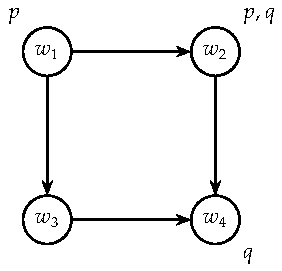
\includegraphics[width=0.4\textwidth]{figures/modal-logic/Kripke-model-basic.pdf}
\caption{Kripke模型的示例}\label{fig:kripke-model-basic}
\end{figure}

模型中,一共有四个可能世界,用$w_1,w_2,w_3,w_4$表示. 他们之间的关系用箭头表示,例如$w_1\to w_2$表示$w_1$到$w_2$有模态算子$\Box$对应的关系. 我们可以把箭头更直观地理解为,从$w_1$这个世界的视角看,他能够想象一个$w_2$的可能世界. 

我们还要指定一个节点作为真实世界,这里我们指定$w_1$作为真实世界. 
\end{example}

我们将节点解读为\textit{可能世界}. 此时,$\Box$被理解为“必然”,$\Diamond$被理解为“可能”. 接下来,我们把模态的语言和模型联系起来,定义模态逻辑的语义,完成模态逻辑三要素的定义. 

设想,在真实世界$w_1$,我们说$\Box p$是真的,换言之,“必然有$p$”. 当我们在说这句话的时候,我们其实在脑中想象了所有能想到的可能世界,然后发现在所有可能世界中,$p$都是真的,于是,我们才说,“必然有$p$”. 这就是模态逻辑的语义. 

形式化地说,$\Box\phi$在世界$w$上成立当且仅当$\phi$在$w$的所有后继上为真. 这种语义通常被称为\textit{Kripke语义}或\textit{可能世界语义}. 在一个世界讨论可能与必然的时候,会取决于它与其他世界的联系. 

我们再来看一个例子. 

\begin{example}\label{ex:kripke-model-basic}
考虑\Cref{fig:kripke-model-basic} 中的Kripke模型. 对哪些$w_i$来说,下式成立?
\[\Box (p\to\Box q).\]
我们以$w_1$为例进行讨论. 其他情况非常类似,读者可以自行验证. 如果$w_1$是真实世界,上要成立上式,必须要所有后继节点上成立
    \[p\to\Box q.\]
$p$的后继节点有$w_2,w_3$,分别考虑这两个节点:
\begin{itemize}
    \item 对于$w_2$,$p$为真,所以需要看$\Box q$是否成立. $w_2$的后继节点只有$w_4$. 注意到,$w_4$上$q$为真,因此$w_2$上$\Box q$成立,所以$w_2$上$p\to\Box q$也成立. 
    \item 对于$w_3$,$p$为假,所以$p\to\Box q$自动成立. 
\end{itemize}
因此,$w_1$上$\Box (p\to\Box q)$成立. 同理,我们可以验证其他节点上的情况,得到在$w_2$,$w_3$,$w_4$上,$\Box (p\to\Box q)$都成立. 

特别注意,在验证$w_4$的时候,因为$w_4$没有后继节点,所以任何命题$\phi$,$\Box\phi$都是成立的. 
\end{example}

游了对概念的自然语言描述和例子,接下来,我们形式上给出模态逻辑的模型和语义定义. 

首先,定义一个\textit{Kripke框架},它单纯描述可能世界及其之间的关系,不考虑可能世界上有哪些命题成立. 

\begin{definition}[Kripke框架]
考虑基本命题模态逻辑$L$. 一个\textbf{Kripke框架}是一个元组$\mathcal F=(W,R)$,其中:
\begin{itemize}
\item $W$是非空集合(可能世界集);
\item $R\subseteq W\times W$是一个$W$上的二元关系(边). 
\end{itemize}
\end{definition}

接下来,对每一个可能世界,我们赋予它为真的原子命题,如此得到了一个\textit{Kripke模型}. 

\begin{definition}[Kripke模型]
一个\textbf{Kripke模型}$\mathcal{M}$是一个元组$(\mathcal F,V)$,其中$\mathcal F$是Kripke框架,$V:\mathbf W\to 2^{\mathbf P}$是\textbf{赋值函数},表示每个可能世界上为真的那些命题字母(即原子命题). 
\end{definition}

Kripke模型并没有指定一个真实世界,接下来,我们引入一个指定的点,作为真实世界,得到\textit{Kripke点模型}. 

\begin{definition}[Kripke点模型]
一个\textbf{Kripke点模型}$(\mathcal{M},w)$是Kripke模型$\mathcal M$加上一个指定的点$w\in W$. 
\end{definition}

以上三个概念的关系如\Cref{fig:kripke-frame-model-point-model} 所示.

\begin{figure}[ht]
\centering
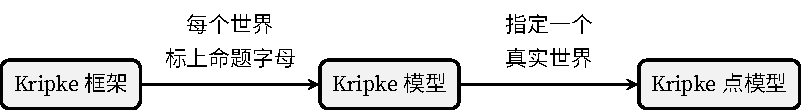
\includegraphics[width=0.95\textwidth]{figures/modal-logic/Kripke-frame-model-point-model.pdf}
\caption{Kripke框架、模型和点模型的关系}\label{fig:kripke-frame-model-point-model}
\end{figure}

现在,我们可以定义模态逻辑的语义,即\textit{Kripke语义}. 

\begin{definition}[Kripke语义]
考虑基本命题模态逻辑$L$. 符号$\mathcal M,w\vDash\phi$表示$\phi$在点模型$\mathcal M,w$是\textbf{可满足的}. 这一概念可以递归定义如下:
\begin{itemize}
\item $\mathcal M, w\vDash\top$永远成立. 
\item $\mathcal M, w\vDash p$当且仅当$p\in V(w)$. 
\item $\mathcal M, w\vDash (\phi\wedge\psi)$当且仅当$\mathcal M,w\vDash\phi$且$\mathcal M,w\vDash\psi$. 
\item $\mathcal M, w\vDash \neg\phi$当且仅当$\mathcal M,w\not\vDash\phi$. 
\item $\mathcal M, w\vDash \Box\phi$当且仅当对所有$v$,如果$wRv$,那么$\mathcal M,v\vDash\phi$. 
\end{itemize}
因此,$\mathcal M, w\vDash \Diamond\phi$当且仅当存在$v$满足$wRv$且$\mathcal M,v\vDash\phi$. 
\end{definition}

注意,上面的定义都是在只有一个模态算子的情况下定义的. 不过,我们可以很容易地推广到多个一元模态算子的情况. 假设模态算子是$\Box_a$,那么Kripke框架中的边需要附上标签$a$,表明这个边是$\Box_a$对应的关系,即$w\to_a v$. 在这种情况下,$\Box_a\phi$的语义定义为:对所有$v$,如果$wR_av$,那么$\mathcal M,v\vDash\phi$. 

多个一元模态算子在知识逻辑中是很常见的. 每个人都有自己对于世界的认知,因此每个人$a$在模型中会有一个对应的关系$R_a$,以描述他所认为的可能世界架构,$R_a$对应的$\Box$模态算子写作$K_a$. 

现在,我们进一步讨论语义的性质. 逻辑公式的语义,无论如何定义,其实都在讨论“什么是真的”这一基本问题. 在模态逻辑中,这一概念尤其复杂. 

比如,在\Cref{ex:kripke-model-basic} 中,我们讨论了$\phi:\Box (p\to\Box q)$在一个Kripke模型中每个可能世界上的真值. 在例子的计算中,我们发现,所有可能世界上$\phi$都是真的. 所以,我们其实可以说,$\phi$在整个Kripke模型上也是真的. 

更进一步,我们也想知道一些关于可能和必然的真理. 为了说明这一点,先回到命题逻辑中,考虑任意命题字母$p$,无论$p$是否是真的,下面这个公式永远都是真的:
\[p\to p.\]
我们在命题逻辑中称这样的公式为\textit{重言式}. 重言式其实反映了命题逻辑的一些根本性质,这些性质独立于具体的命题而存在. 比如\textit{排中律}:对于任意命题$p$,$p\vee\neg p$是重言式,再比如\textit{三段论}:$((p\to q)\wedge p)\to q$是重言式. 他们是我们做逻辑推理的时候自动会假设的性质. 

同样的问题也可以对模态逻辑提出:有没有一些关于可能和必然的性质,是独立于具体的可能世界而存在的?比如,我们是否可以说,如果$p$是真的,那么$p$必然是真的?把它写成模态逻辑的形式就是:
\[p\to \Box p.\]
如果这是一个关于必然的真理,那么,无论$p$是否为真,无论我们处于什么样的可能世界,这个公式都应该是真的. 

根据上面的启发,在模态逻辑的体系中,我们可以定义各种不同粒度的“真”的概念:

\begin{definition}[模态逻辑的真值]
给定模态逻辑公式$\phi$,我们可以定义它的真值:
\begin{itemize}
\item $\phi$在点模型$\mathcal M,w$\textit{可满足}指的是$\mathcal M,w\vDash \phi$. 
\item $\phi$在模型$\mathcal M$\textit{有效},记为$\mathcal M\vDash \phi$,指的是$\mathcal M,w\vDash\phi$对所有$w$成立. 
\item $\phi$在点框架\footnote{我们在前文中没有定义点框架,但是点框架的定义相当直接:它是一个Kripke框架加上一个指定的点. }$\mathcal F,w$\textit{有效},记为$\mathcal F,w\vDash \phi$,指的是$\mathcal M,w\vDash\phi$对所有基于$\mathcal F$的模型$\mathcal M$成立. 
\item $\phi$在框架$\mathcal F$\textit{有效},记为$\mathcal F\vDash \phi$,指的是$\mathcal M\vDash\phi$对所有基于$\mathcal F$的模型$\mathcal M$成立. 
\item $\phi$对框架类(即框架的一个集合)$K$\textit{有效},记为$\vDash_K\phi$,指的是$\mathcal F\vDash\phi$对所有$\mathcal F\in K$成立. 
\end{itemize}
\end{definition}

我们可以看到,模态逻辑的真值有两个维度的粒度:局部-全局,模型-框架. 越靠左边的真值越具体,越靠右边的真值越一般. 我们可以用下面的表格来总结这些概念:
\[\begin{array}{c|cc}
\toprule
 & \text{模型} & \text{框架} \\ \midrule
\text{局部} & \light{\mathcal M,w\vDash \phi} & \mathcal F,w\vDash \phi \\
\text{全局} & \mathcal M\vDash \phi & \light{\mathcal F\vDash \phi} \\
\bottomrule
\end{array}\]
我们主要讨论高亮的两个部分. 

左上角反映了某个具体可能世界结构中的某个具体世界上的真值. 例如,假设$p$表示“地球是球形的”,那么在我们所生活的这个世界上,$p$是真的,但是,我们的确可以想象出来另一个可能世界,地球是平的,那么在这个可能世界上,$p$是假的. 因此,这是一个只适用于我们所生活的这个可能世界的真值.

右下角反映了某个具体框架中所有可能世界上的真值. 例如,考虑命题$\phi:p \to\Diamond p$表示“如果$p$是真的,那么可能$p$是真的”. 这是一个关于可能的陈述,看起来是非常合乎道理的. 我们无法想象出一个可能世界,$p$是真的,但不可能$p$是真的. 所以,如果$\mathcal{F}$表示“可能”所对应的框架,那么$\phi$在$\mathcal{F}$上是有效的. 然而,如果$\Diamond$被理解为“相信”,$\phi$就完全没有任何道理. 因而,在“相信”所对应不同的框架$\mathcal{F}'$上,$\phi$不再有效.

因此,从左上角到右下角的过程,是从具体、特定的真值到一般、普遍的真值的过程.

更抽象地来看,\Cref{ex:kripke-model-basic} 其实给出了左上角的一个例子,下面,我们可以演示右下角的一个例子. 

\begin{example}\label{ex:modal-logic-frame-validity}
考虑\Cref{fig:frame-validity} 中的框架,它是\Cref{fig:kripke-model-basic} 中的Kripke模型去掉了命题字母的结果. 
\begin{figure}[ht]
\centering
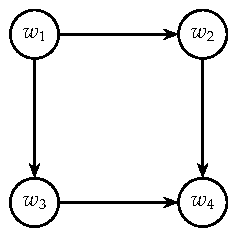
\includegraphics[width=0.35\textwidth]{figures/modal-logic/frame-validity.pdf}
\caption{框架语义的示例} \label{fig:frame-validity}
\end{figure}

我们问,对于这个框架,下面的公式是否有效?
\[\Box (p\to\Box p).\]
为此,我们需要考虑四个可能世界上的情况. 同样,我们只对$w_1$进行讨论,其他情况类似. 对于$w_1$,有两个后继节点$w_2$,$w_3$,我们需要验证$p\to\Box p$在这两个节点上是否成立. 

先考虑$w_2$,假设$p$在$w_2$上为真,我们需要验证$\Box p$是否成立. $w_2$的后继节点只有$w_4$,但我们可以让$p$在$w_4$上为假,这样$\Box p$就不成立. 因此,$w_2$上$p\to\Box p$也不成立,从而$w_1$上$\Box (p\to\Box p)$不成立. 

于是,我们找到了一种赋值的方案,使得$\Box (p\to\Box p)$在$w_1$上不成立. 因此,这个公式在整个框架上也不有效. 
\end{example}


最后,我们说明,上面的讨论在知识逻辑中都是自然成立的. 此时,模态公式$K_i\phi$被读作“$i$知道$\phi$”. 从语义来说,$K_i$是$\Box$算子,即我知道$\phi$意味着在我认为的所有可能世界中$\phi$都是真的,即:
\[
\mathcal M,w\vDash K_i\phi\Longleftrightarrow\text{对任意$v$,如果$w\to_i v$,那么$\mathcal M,v\vDash\phi$}. 
\]
同样,模态公式的真值有两个层面:
\begin{itemize}
\item 在点模型上可满足:$\mathcal M,w\vDash\phi$;
\item 在框架上有效:$\mathcal F\vDash\phi$. 
\end{itemize}

\section{模态可定义性}\label{sec:modal-definability}

逻辑的意义在于把对事物的抽象认知用形式化的语言表述出来. 我们已经看到,我们对事物的认知可以被两种方式描述出来:一是通过Kripke模型(框架)的特殊结构,二是通过具体的模态公式. 那么,这两种方式之间有什么联系呢?本节我们研究这个问题. 

先看几个例子. 
\begin{example}
考虑知识逻辑,假设只有一个知识算子$K$. 设有命题$p$,如果$p$是真的,那么我不知道非$p$,即$\phi: p \to \neg K \neg p$. 这是用逻辑表述了关于知道的一种性质. 

另一方面,我们也可以将对于$K$的理解反映到Kripke模型中. 一个合理的性质是:真实世界是我能够感知到的可能世界. 换言之,对任何$x$,都有$xRx$,这是一个自反关系. 在这种情况下,容易验证,对于自反点模型以及框架$\mathcal{F}$,我们有$\mathcal{M}, v \vDash \phi$以及$\mathcal{F} \vDash \phi$. 
\end{example}

上面的例子说明,对于特定的公式,它会在某类模型上成立. 反过来,我们也可以讨论,成立特定公式的模型是什么样的,我们看下面的例子. 

\begin{example}\label{ex:box-top}
考虑基础模态逻辑和它的公式$\Diamond \top$. 对于一个Kripke点模型$\mathcal{M},w$,假设$\mathcal{M}, w \vDash \Diamond \top$,我们来研究$\mathcal{M}$的特殊性质. 

根据定义,这意味着存在一个点$v$,使得$w R v$并且$\mathcal{M}, v \vDash \top$,由于后一半永远成立,所以,这等价于$w$有一个后继. 同样的,对于任意框架$\mathcal{F}$,如果$\mathcal{F} \vDash \Diamond \top$,则基于$\mathcal{F}$的每个点模型$\mathcal{M}, v$都满足$\Diamond \top$,即$\mathcal{F}$的每个点都有后继. 
\end{example}

上面两个例子说明了模型性质和模态公式之间单向的联系,下面的例子说明,这种联系也可以是双向的. 

\begin{example}
考虑公式$\phi:p \to \Diamond p$. 我们研究和这个公式完全对应的框架$\mathcal{F}$的性质. 
\begin{itemize}
    \item 任给一个赋值$V$和点$w$都有$\mathcal{M}, w \vDash p \to \Diamond p$. 考虑一个赋值$V$,使得只有$w$上有$p$. 因为$w$上有$p$,为了使$\phi$成立,$w$必须要有一个后继上也有$p$. 在我们的这个赋值下,这意味着$w$必须以自己为后继. 因此,对任意$w$,$wRw$成立,即$\mathcal{F}$是一个自反框架. 
    \item 反过来,如果$\mathcal{F}$是一个自反框架,那么对于任意赋值$V$和点$w$,容易验证$\mathcal{M}, w \vDash p \to \Diamond p$. 因此,$\mathcal{F} \vDash p \to \Diamond p$. 
\end{itemize}
结合这两点,我们可以说,$p\to \Diamond p$定义了自反框架. 

此外,结合这个例子与\Cref{ex:box-top},我们会发现,一个框架的特定性质可以由多个不同的公式定义. 
\end{example}

以上例子给我们启示,我们可以用模态公式去定义模型或框架的性质. 这种定义被称为\textit{模态可定义性},我们给出如下定义. 

从点模型的角度,我们可以讨论模态公式定义了什么样的点模型. 

\begin{definition}[点模型可定义性]
设$\mathcal{K}$是一些点模型的集合,$\Sigma$是一些模态公式的集合. 我们说\textbf{$\mathcal{K}$可由公式集$\Sigma$定义},指的是对于任意点模型$\mathcal{M}, w$,$\mathcal{M}, w \in \mathcal{K}$当且仅当对任意$\phi\in\Sigma$,
\[ \mathcal{M}, w \vDash \phi. \]

如果$\Sigma = \{\phi\}$,我们就说\textbf{$\mathcal{K}$可以由公式$\phi$定义}. 
\end{definition}

我们也可以从框架的角度讨论模态可定义性,定义类似. 

\begin{definition}[框架可定义性]
设$\mathcal{K}$是一些框架的集合,$\Sigma$是一些模态公式的集合. 我们说\textbf{$\mathcal{K}$可由公式集$\Sigma$定义},指的是对于任意框架$\mathcal{F}$,$\mathcal{F} \in \mathcal{K}$当且仅当对任意$\phi\in\Sigma$,
\[ \mathcal{F} \vDash \phi. \]

如果$\Sigma = \{\phi\}$,我们就说\textbf{$\mathcal{K}$可以由公式$\phi$定义}. 
\end{definition}

\begin{remark}
    关于模态逻辑更系统性的论述,请参见教材~\cite{blackburnModalLogic2001}、Stanford哲学百科~\cite{garsonModalLogic2024},此外,课程~\cite{WangYanJingAdvancedModalLogic} 也是一个很好的资源. 关于模态逻辑在更广泛领域中的应用,可以参考van Benthem的著作~\cite{benthemModalLogicOpen2010}.
\end{remark}

\section{知识逻辑的基本模型与性质}\label{sec:epistemic-logic-basic-model}

接下来,我们将注意力放在知识逻辑上,将前面若干小节讨论的概念应用到知识逻辑中. 

\subsection{知识逻辑的Kripke模型与公理}

首先,从模型的角度看,一个自然的假设是,对每个个体$i$来说,他认为的可能世界之间应该是不可区分的. 这意味着,对于每个个体$i$,他认为的可能世界之间的关系$R_i$应该是等价关系,我们记作$\sim_i$:

\begin{itemize}
    \item 自反:$\forall x,x\sim_ix$. 我能够想象到真实的世界. 
    \item 传递:$\forall x,y,z(x\sim_iy\wedge y\sim_iz)\to x\sim_iz$. 如果我在$x$世界能够想象到$y$世界,在$y$世界能够想象到$z$世界,那么我在$x$世界也能够想象到$z$世界. 
    \item 对称:$\forall x,y(x \sim_i y\leftrightarrow y\sim_ix)$. 我能够在$x$世界想象到$y$世界,那么我也能够在$y$世界想象到$x$世界. 
\end{itemize}
我们将$R_i$是等价关系的框架类记为$H$. 

从模态可定义性的角度来说,$\sim_i$ 的特殊性质会对应 $K_i$ 特殊的公式. 这些公式就可以被看成关于“知道”的公理或推导规则. 承认某一条公理或推导规则就必须承认可能世界具有某一种性质,反之亦然. 

接下来,我们给出知识逻辑的基本性质,即公理. 

\begin{proposition}[分配公理]
$\vDash (K_i(\phi\to\psi)\wedge K_i\phi)\to K_i\psi$.
\end{proposition}

\begin{proof}
假设 $\mathcal M,w\vDash K_i(\phi\to\psi)$ 且 $\mathcal M,w\vDash K_i \phi$. 于是,对所有 $R_i$ 后继 $v$ 都有 $\mathcal M,v\vDash\phi\to\psi$ 和 $\mathcal M,v\vDash\phi$,因而 $\mathcal M,v\vDash\psi$. 根据定义,$\mathcal M,w\vDash K_i\psi$,因而对所有 $\mathcal F$,分配公理有效. 
\end{proof}

分配公理意味着拥有知识的个体可以对自己的知识做任意的演绎推理,因而假设个体是\textit{逻辑全知的}. 注意,分配公理并没有用到框架类$H$的性质,所以,它其实是模态逻辑的一个普适公理. 

\begin{proposition}[泛化规则]
对所有 $\mathcal F$,如果 $\mathcal F\vDash\phi$,那么 $\mathcal F\vDash K_i\phi$. 
\end{proposition}

\begin{proof}
假设 $\mathcal F\vDash\phi$,这意味着对所有基于 $\mathcal F$ 的点模型都有 $\mathcal M,w\vDash\phi$. 因此,对任意 $w$ 的 $R_i$ 后继 $v$,也有 $\mathcal M,v\vDash\phi$. 所以也有 $\mathcal M,w\vDash K_i\phi$ 成立,因而 $\mathcal F\vDash K_i\phi$. 
\end{proof}


泛化规则可能不太容易理解,我们举一个例子. 生活在中国,我们都知道农历五月初五是端午节,“五月五,迎端午”,按照传统习俗要吃粽子. 这意味着,在我们所有对未来生活的设想中,“农历五月五要吃粽子”这一习俗是牢固存在的. 因此,对于中国人来说,我们身处的世界以及幻想的可能世界组成了框架$\mathcal F$,而“农历五月五吃粽子”是这个框架中的一个普适规律. 

然而,如果我们生活在冰岛,一个中国人非常少的国家,那么,“农历五月五要吃粽子”这一习俗可能就不再广为流传. 在这种情况下,我们所处的世界及想象的可能世界组成了另一个框架$\mathcal F'$,在这个框架中,“农历五月五要吃粽子”不再是普适规律. 

所以,泛化规则其实在说,如果$\phi$是$\mathcal F$普遍适用的规律,不依赖具体的命题,那么我就知道$\phi$. 当然,这个规律$\phi$可能只适用于$\mathcal F$. 但无论如何,我清晰地知道这个世界的运作规律. 特别地,我知道关于知识的这些规律. 

同样,泛化规则也没有使用框架类$H$的性质,所以它也是模态逻辑的普适规则. 

\begin{proposition}[知识公理,真理公理]\label{prop:knowledge-axiom}
$\vDash_H K_i\phi\to\phi$.
\end{proposition}

注意,从知识公理开始,我们就开始使用了框架类$H$的性质. 从这里开始的性质,和\Cref{chap:bayesian-game}中讨论的知识的性质是一致的,所以这里不再赘述. 他们的证明类似前述性质,这里不再给出,见习题 \ref{exercise:epistemic-logic-axioms}.

\begin{proposition}[内省公理]\label{prop:knowledge-introspection}
正内省公理:
\[\vDash_H K_i\phi\to K_iK_i\phi.\]

负内省公理:
\[\vDash_H \neg K_i\phi\to K_i\neg K_i\phi.\]
\end{proposition}

以上五条性质(四条公理+一条推导规则)加上 MP 形成的推理系统称为 \textit{S5 公理系统}. 需要注意的是,这些公理其实都是公理模式,对每一个具体的命题$\phi$,都有一条公理,因此,它其实包含了无穷条公理. 

从哲学的角度讨论,还有一些别的公理. 

\begin{proposition}[一致性公理]\label{prop:knowledge-consistency}
$\vDash_H\neg K_i\bot$.
\end{proposition}

因此,个体不能够知道假的陈述,以此区别于信念. 

我们基于框架类 $H$ 给出了关于知识的公理. 反过来,公理对应什么样的框架结构呢?我们总结于\Cref{tab:epistemic-axiom-structure}.

\begin{table}[ht]
\centering
    \begin{tabular}{c|c}
        \toprule 公理 &  $R_i$ 的性质 \\
        \midrule $K_i \varphi \to \varphi$ & 自反性 \\
        $K_i \varphi \to K_i K_i \varphi$ & 传递性 \\
        $\neg K_i \varphi \to K_i \neg K_i \varphi$ & Euclid性 \\
        $\neg K_i\bot$  & 序列性\\
        $\varphi \to K_i \neg K_i \neg \varphi$ & 对称性 \\
        \bottomrule
    \end{tabular}
    \caption{知识公理对应的框架结构} \label{tab:epistemic-axiom-structure}
\end{table}

表中有两个性质是我们没有讨论过的,这里给一个简短的解释. 
\begin{itemize}
    \item Euclid性:$\forall x,y,z(xR_iy\wedge xR_iz\to yR_iz)$,也就是说,关系一定形成三角形. 
    \item 序列性:$\forall x\exists y\, xR_iy$,所有点都有后继. 
\end{itemize}

以上的模态可定义性和\Cref{sec:modal-definability}中的例子类似,这里不再给出,请见习题 \ref{exercise:epistemic-logic-axiom-structure}.

可以看出来,以上关系其实并不是孤立的,我们有以下引理:

\begin{lemma}\label{lemma:relation-properties}
\begin{itemize}
    \item 如果 $R_i$ 是自反和Euclid的,那么 $R_i$ 是对称和传递的.
    \item 如果 $R_i$ 是对称和传递的,那么 $R_i$ 是Euclid的.
    \item 以下命题等价:
    \begin{itemize}
        \item $R_i$ 是自反、对称和传递的.
        \item $R_i$ 是对称、传递和序列的.
        \item $R_i$ 是自反和Euclid的.
    \end{itemize}
\end{itemize}
\end{lemma}

这一性质的验证根据定义即可,见习题 \ref{exercise:relation-properties}.

下面我们向知识逻辑语言中加入共同知识算子和它的语义. 首先加入“所有人都知道”这个算子:
\[E\phi\leftrightarrow\bigwedge_i K_i\phi.\]
记 $E^k\phi$ 为 $\underbrace{E\dots E}_k\phi$. 于是,我们可以给共同知识算子一个语义定义:

\begin{definition}[共同知识算子]
\textbf{共同知识算子} $C$ 的语义定义为:
\[
\mathcal M,w\vDash C\phi\iff\mathcal M,w\vDash E^k\phi,\quad k=1,2,\dots
\]
\end{definition}

我们可以从图结构来理解共同知识算子. 把所有边上的标记忽略掉,Kripke模型变成一个有向图,节点上的标记是这个节点上成立的原子命题. 于是,我们有如下解读:
\begin{itemize}
    \item $\mathcal M,w\vDash E^k\phi$的含义是,从$w$出发走恰好$k$步可到达的可能世界$v$上都有$\mathcal M,v\vDash \phi$. 这一解读的示意见\Cref{fig:Ek-illustration},
    
    在这个图中,$\mathcal M,w_1\vDash E^3\phi$,因为从$w_1$出发,经过三步可以到达的可能世界上都有$\mathcal M,v\vDash \phi$,我们具体地标出了两条图路径:$w_1\to_1 w_2\to_3 w_3\to_1 w_5$对应$K_1K_3K_1\phi$,$w_1\to_2 w_4\to_2 w_3\to_2 w_6$对应$K_2K_2K_2\phi$.
    \item 因此,$\mathcal M,w\vDash C\phi$的含义便是,从$w$出发经过有限步可到达的可能世界$v$上都有$\mathcal M,v\vDash \phi$.
\end{itemize}
\begin{figure}[ht]
    \centering
    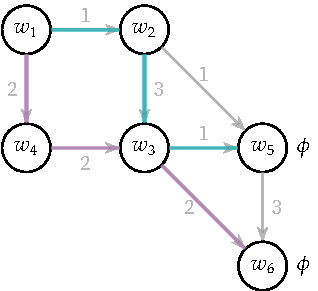
\includegraphics[width=0.5\textwidth]{figures/modal-logic/Ek-illustration.pdf}
    \caption{$\mathcal M,w_1\vDash E^3\phi$的示意图,我们标出了其中的两条路径.} \label{fig:Ek-illustration}
\end{figure}

接下来,我们给出共同知识算子的性质. 实际上,共同知识算子可以充分必要地被下面两个公理所定义(验证见习题 \ref{exercise:common-knowledge-axioms}):

\begin{proposition}[不动点公理]\label{prop:common-knowledge-fixed-point}
\[\vDash C\phi\leftrightarrow E(\phi\wedge C\phi).\]
\end{proposition}

\begin{proposition}[归纳规则]\label{prop:common-knowledge-induction}
如果
\[\mathcal F\vDash \phi\to E(\phi\wedge\psi),\]
那么 
\[\mathcal  F\vDash \phi\to C\psi.\]
\end{proposition}

现在我们来讲解上面两个公理的含义. 

不动点公理是比较直接的. 什么是共同知识?对任意$k$,$E^k\phi$成立. 我们把不动点公理展开,可以得到:
\begin{align*}
    C\phi&\leftrightarrow E(\phi\wedge C\phi)\\
    &\leftrightarrow E\phi\wedge E(C\phi)\\
    &\leftrightarrow E\phi\wedge E(E\phi\wedge E(C\phi))\\
    &\leftrightarrow E\phi\wedge E^2\phi\wedge E^3(C\phi)\\
    &\dots
\end{align*}
因为逻辑公式不允许写无穷长的公式,所以,不动点公理就是在用一个算子的\textit{递归方程}来定义共同知识:
\[\forall\phi,C\phi\leftrightarrow E(\phi\wedge C\phi). \]

然而,一个递归方程可能会有无穷多个解,并不是所有的解都是我们要的那个. 所以,归纳规则给出了共同知识算子的另一个性质:这是这个递归方程的\textit{最小解}. 下面我们来说明这一点. 

我们先从一个看似无关的例子讲起. 用数学归纳法证明一个关于自然数的命题$P(n)$时,我们需要两个步骤:
\begin{itemize}
    \item 证明基础情形$P(0)$成立;
    \item 证明归纳步骤:如果$P(n)$成立,那么$P(n+1)$也成立. 
\end{itemize}
因此,归纳的思想是,我们先找到一个基础情形,然后一点一点把成立的集合扩大,直到包含所有的情况. 

注意,在真正的证明中,我们不能真的把每一个$P(n)$的正确性都从更小的情况推导出来,因为这是无穷多个情况. 实际上,我们写归纳法证明的过程中,隐含地写了一个关于$P$的递归方程,左边是这个一点一点扩大的过程,右边是我们要证明的命题:
\begin{align*}
    (P(0)\wedge\forall n,(P(n)\to P(n+1)))\leftrightarrow\forall n,P(n).
\end{align*}
所以,数学归纳法就是一个公理,它说明这样一点一点扩大的过程(左边)的确可以用来证明所有的情况(右边). 注意,这个公理产生的$P$是递归方程的\textit{最小解},因为它是从最小情况逐步扩大得到的结果. 

回到共同知识算子$C$,其实$C$和数学归纳法里的证明$P$的过程是非常相似的. 它的定义也是从基础情形$\phi$开始,然后一点一点扩大,每次扩大都是用$E$算子,直到无穷层. 因此,它也具有归纳的性质. 

观察归纳规则,它的前提条件是:
\[\mathcal F\vDash \phi\to E(\phi\wedge\psi).\]
这一个步骤描述了,如果我们已经构造了$\phi$,我们如何用$E$算子构造下一层的命题. 这就相当于数学归纳法中从$P(n)$到$P(n+1)$的过程. 

而归纳规则的结论是:
\[\mathcal  F\vDash \phi\to C\psi.\]
这个结论说明,如果我们可以逐层加$E$算子,那么这个叠加可以无穷进行下去,最终得到的就是$C$算子. 这就相当于数学归纳法中证明$P(n)$对整个自然数集成立. 

所以,上面的类比说明了归纳规则的含义:它确保了$C$算子是递归方程的最小解,也就是那个逐层叠加$E$所定义的算子. 

\begin{remark}
    关于不动点的这种理解,实际上源自对归纳法和余归纳法的研究,这是类型论和模态逻辑中的一个重要思路. 关于这一点,可以参见类型论和编程语言相关的教材,例如~\cite{pierceTypesProgrammingLanguages2002,pierceSoftwareFoundationsVolume,avigadTheoremProvingLean}. 此外,在模态逻辑社区也有所谓\textit{$\mu$-演算}的研究,这是一个专门研究递归方程的形式化方法~\cite{kozenResultsPropositionalMcalculus1982}. 还有一些数学中的例子~\cite{abdelgawadInductionCoinductionFixed2019}、哲学中的例子~\cite{linneboPredicativeImpredicativeDefinitions} 可以参考. 
\end{remark}

最后,将 S5 公理系统中加入关于 $E$ 和 $C$ 的公理,我们就扩展了知识逻辑. 因为 $E$ 和 $C$ 是用 $K_i$ 定义的,因此它们本身并不会带来 Kripke 模型新的结构性质. 

\subsection{Kripke模型与Aumann结构}

Kripke模型与Aumann结构之间存在着非常本质的对应关系. 
\begin{itemize}
    \item 在Kripke模型中,我们将算子$K_i$对应的关系限制为了等价关系,因为我们希望$i$想象的可能世界之间是不可区分的. 
    \item 在Aumann结构中,我们将$i$的信息集定义了全集的一个划分,把每个划分作为他的原子信息. 
\end{itemize}

上面的两个概念实际上是可以相互转换的. 数学上说,等价关系充分必要地给了集合一个划分;从概念上说,所谓不可区分,就是原子性. 因此,他们之间其实存在一一对应的关系. 

进一步,如果回忆\Cref{chap:plausible-reasoning}的思想,我们可以看到逻辑与集合之间的联系如\Cref{tab:Kripke-Aumann} 所示. 

\begin{table}[ht]
    \centering
    \begin{tabular}{c|c}
    \toprule
    Kripke模型 & Aumann结构 \\
    \midrule
    可能世界 & 样本点 \\
    公式 & 事件 \\
    原子命题 & 基本事件 \\
    模态算子 & 集合-集合映射 \\
    $i$的等价关系 & $i$的划分 \\
    逻辑连接词 & 集合操作 \\
    \bottomrule
    \end{tabular}
    \caption{Kripke模型与Aumann结构的对应关系} \label{tab:Kripke-Aumann}
\end{table}

实际上,在S5公理系统下,这种对应关系可以被严格地叙述和证明,见习题 \ref{S5-Aumann-equivalence}.

Kripke模型和Aumann结构的一个重要区别在于它们各自的研究偏好:Kripke语义偏重于逻辑,而Aumann结构则偏重于(Bayes)概率论. 因此,用数学来研究知识论可以呈现出两种风格:一种是计算机科学、逻辑学和哲学的风格,另一种则是经济学和信息论的风格. 

然而,这种对应关系完全依赖于我们对知识的基本假设:
\begin{itemize}
    \item 对于Kripke模型,我们假设了知识满足S5公理系统;
    \item 对于Aumann结构,我们假设了知识满足\eqref{eq:K0-awareness}--\eqref{eq:K4-negative-introspection}. 
\end{itemize}
如果这些假设被打破,那么这样的对应关系就不再成立. 例如,如果我们移除负自省公理,Kripke模型就不再具备等价关系的性质,因此不再能够对应于Aumann结构中的信息集. 

从对知识刻画精细程度来说,两种研究方法也有区别. 通常来说,Aumann结构要想破坏某一条性质是非常难的,因为它是基于概率论和事件的概念. 然而,Kripke模型具有(模态)逻辑的风格,因此,研究加入或者去除某个公理带来的影响是它最“正统”的研究方法. 


\subsection{“泥泞的孩童”再回顾:形式化解法}

作为一个具体的例子,我们现在把\Cref{chap:bayesian-game}中的“泥泞的孩童”问题用知识逻辑的语言来重新讨论. 我们终于可以用形式化的方式来严格讨论这一问题了. 

我们要给出“泥泞的孩童”的逻辑三要素. 首先,语言就是知识逻辑语言. 然后,我们给出Kripke模型以及对应的语义. 

可能世界可以表示为$\{0,1\}^n$的元素$x=(x_1,\dots,x_n)$,其中$x_i=1$表示孩子$i$的脸上有泥巴,$x_i=0$表示$i$的脸上没有泥巴. 我们假设每个孩童$i$的可达关系$R_i$都是一个等价关系. 在这种假设下,每个孩子唯一不是共同知识的事情就是他们脸上泥巴的状态,而其他所有事情都被隐含在了Kripke模型之中. 

接下来,我们给出命题字母:原子命题$p_i$表示孩子$i$脸上有泥巴,命题$p$表示至少有一个孩子脸上有泥巴. 

假设现在父亲还没有宣布$p$. 对于孩子$i$来说,他的认知中只有两个可能世界:一个是他的脸上有泥巴,另一个是他的脸上没有泥巴. 其他对他来说都是确定的. 因此,有$x R_i y$当且仅当$x_j=y_j$对于任意$j\neq i$成立. 在这种情况下,框架$\mathcal{F}$对应于一个$n$维超立方体. 

例如,当$n=3$时,框架$\mathcal{F}$对应的立方体结构如\Cref{fig:modal-logic-cubic} 所示. 

\begin{figure}[ht]
    \centering
    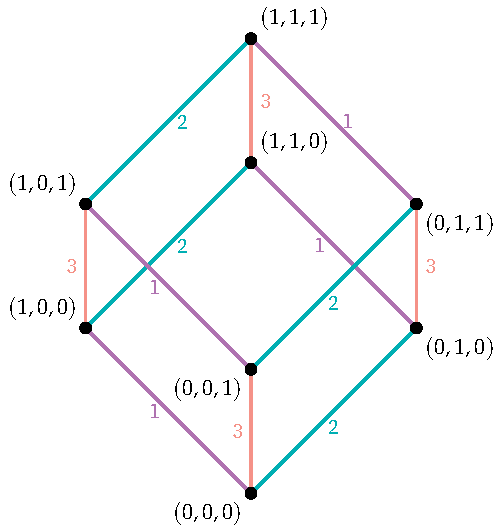
\includegraphics[width=0.6\textwidth]{figures/modal-logic/cubic-example.pdf}
    \caption{“泥泞的孩童”问题的Kripke模型}\label{fig:modal-logic-cubic}
\end{figure}

从框架$\mathcal{F}$到模型$\mathcal{M}$,我们还需要确定赋值$V$. 
\begin{itemize}
    \item 对任意$p_i$和$w$,有$w\in V(p_i)$当且仅当$w_i=1$;
    \item $p\in V(w)$当且仅当$w$的所有分量$w_j$不全为零. 
\end{itemize}

从模型到点模型,我们还需要确定我们所处的可能世界,从而可以讨论模态公式的可满足性. 例如:$\mathcal{M},(1,0,1)\vDash Ep$,但是$\mathcal{M},(1,0,1)\vDash \neg E^2p$. 

假设父亲宣布了$p$,那么框架$\mathcal{F}$将会发生变化,如\Cref{fig:modal-logic-cubic-after-father} 所示. 

\begin{figure}[h]
    \centering
    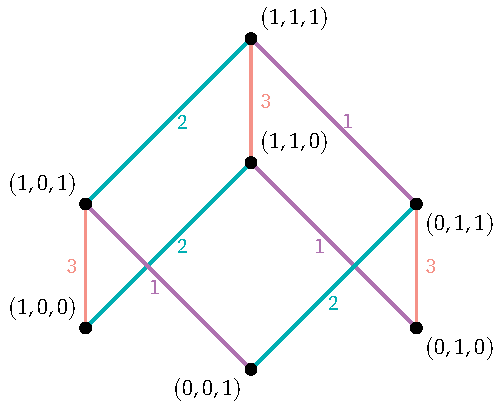
\includegraphics[width=0.6\textwidth]{figures/modal-logic/cubic-example-after-father.pdf}
    \caption{父亲宣布$p$之后的Kripke模型}\label{fig:modal-logic-cubic-after-father}
\end{figure}

在$i$的认知中,只有两个可能世界. 因此,$i$回答“知道”意味着她能够确定只有一个世界;她回答“不知道”意味着还有两个可能世界. 

假如现在是第一轮问答,如果所有人都回答了“不知道”,考虑状态$s=(1,0,0,\dots)$. 如果真实世界是$s$,那么对于$1$来说,可能世界只有一个了,但她却说“不知道”,这说明真实世界不是$s$. 同理,所有只有一个$1$的可能世界都会被排除. 由此可以归纳得出,第$k$轮的时候,所有只有$k$个$1$的可能世界都会被排除. 

然而,如果父亲没有宣布$p$,那么$\mathcal{M}$是一个超立方体. 在任何一轮中,每个孩子都会认为有两个可能世界,因此不会有任何可能世界被排除. 

因此,从结构上来说,父亲宣布$p$改变了每个孩子对应的$R_i$等价的可能世界,使得一些孩子可以确定自己所处的世界. 因而,父亲宣布$p$之后,孩子们的回答会有本质不同. 

实际上,这一套方法可以将类似的智力谜题用算法化的方式得到解答,这是知识逻辑的一个有趣的应用. 这是早年的人工智能研究最为热衷的几个方向之一(见\Cref{chap:information-theory}的章首引言). 

\section{对不一致达成一致}

作为一个更正式的(也更更复杂!)例子,本节将用模态逻辑的方式来探讨达成一致与共同知识的关系,这个问题最早由Aumann提出~\cite{aumannAgreeingDisagree1976}. 在AI时代的版本是:两个拥有相同决策规则的AI是否会进行交易?如果交易发生,这意味着买家和卖家采取了不同的决策(一个购买,一个出售);否则,他们将不会达成交易. 

我们将证明,对于有相同决策方式的两个个体,他们不可能对采取不同行动这件事具有共同知识. 因此,如果两个AI按照相同的规则行事,交易便不会发生. 一句话概括,\
\begin{quotation}
    玩家不能“对不一致达成一致”(agree to disagree). 
\end{quotation}

\subsection{模型}

下面,我们开始介绍这个模型. 

首先,我们介绍一下二人博弈的模型. 这个模型是一个无随机性的Markov博弈,详细讨论见\Cref{sec:stochastic-game}. 设有两个玩家1和2,在任意时刻,每个玩家处于某个局部状态$s_i$之中,局部状态空间分别记为$S_1$和$S_2$. 整个系统的全局状态为$(s_1, s_2) \in S_1 \times S_2 = \mathcal{G}$. 

接下来,我们描述博弈的整个过程. 用非负整数$m$来表示当前时刻,初始时刻为$0$. 系统的一次\textit{运行}是一个函数$r: m \mapsto (s_1, s_2)$,描述了系统每一时刻的全局状态. $\mathcal{R}$是全局状态空间$\mathcal{G}$上的所有可能运行的集合. 对于每个运行$r \in \mathcal{R}$,$(r, m)$被称为系统$\mathcal{R}$的一个\textit{点}. 

玩家处于某个状态时,可以采取某种行动. 为了反映“玩家按照相同的规则行事”,我们规定两个玩家的行动集相同,记为$A$,且这一行动集不依赖于全局或局部状态. 给定所有人的行动和一个全局状态,系统的\textit{转移函数}$\tau: A^2 \times \mathcal{G} \to \mathcal{G}$描述了如何从一个状态转移到另一个状态. 

为了描述“按照规则行事”,我们引入\textit{策略}的概念. 玩家$i$的策略$P_i$是从局部状态$S_i$到行动集$A$的映射,即根据状态采取行动. 两个玩家的策略组合记为$P = (P_1, P_2)$. 这是Markov博弈的一种限制,我们要求玩家的策略只依赖于自己的状态,并且不允许随机行动. 

策略的执行需要初始状态. 初始状态可能的集合记为$\mathcal{G}_0$. 给定初始状态集$\mathcal{G}_0$和转移函数$\tau$,我们就可以在系统上执行任何一种策略. 我们称元组$\gamma = (\mathcal{G}_0, \tau)$为系统的\textit{上下文}. 

给定上下文$\gamma = (\mathcal{G}_0, \tau)$和一个策略组合$P$,整个系统就可以运行起来了,产生一个运行. 不难看出,给定一个运行$r$,它与策略$P$\textit{相容}的条件为:
\[
r(0) \in \mathcal{G}_0, \quad \forall m,\ r(m+1) = \tau(P(s_1), P(s_2))(r(m)),
\]
其中$r(m) = (s_1, s_2)$. 换言之,$r$是从某个可能的初始状态开始执行策略$P$产生的运行. 系统$\mathcal{R}$表示上下文$\gamma$和策略组合$P$,其包含的所有运行$r$都与$P$相容. 我们用$\mathcal{R}^{rep}(P, \gamma)$表示这样的系统. 

以上我们就完成了博弈部分的建模. 接下来,我们引入逻辑部分的建模,并把它与博弈的部分对应起来. 

首先,我们引入Kripke模型. Kripke模型的点是系统的点. 然后是原子命题集$\mathbf{P}$. 它的元素形如$perf_i(a)$,表示玩家$i$采取行动$a$. 

我们还需要定义赋值函数$V$,它将Markov博弈中的概念和原子命题联系起来. 具体来说,定义如下:原子命题$perf_i(a)\in V(s)$当且仅当在状态$s$玩家$i$采取了行动$a$. 

然而,赋值函数的定义域应该是一个Kripke模型中的点,这个点不同于Markov博弈中的状态. 因此,我们需要将赋值函数扩展到系统的点集:$p \in V((r, m))$当且仅当$p\in V(r(m))$. 

随后,我们引入知识算子$K_i$,假设$K_i$对应的等价关系是$\sim_i$. 玩家$i$只能区分自己的局部状态$s_i$,即
\[(r, m) \sim_i (r', m')\iff r(m)_i = r'(m')_i.\]
根据Aumann结构,局部状态$s_i$对应的信息集为
\[
IS_i(s_i, \mathcal{R}) = \{(r, m): r \in \mathcal{R}, r(m) = s_i\}.
\]
如此一来,我们得到了Kripke点模型$\mathcal{M}, (r, m)$以及知识算子$K_i$.

此外,除了知识算子,Markov博弈还有时间的概念,因此我们引入时间模态算子$X$,表示“下一时刻”. 其语义定义为:
\[
\mathcal{M}, (r, m) \vDash X\phi \iff \mathcal{M}, (r, m+1) \vDash \phi.
\]
利用算子$X$,我们可以用公式$act_i(a)$表示“$i$将要采取行动$a$”:
\[act_i(a) \leftrightarrow \neg perf_i(a) \wedge X perf_i(a).\]

最后一步,为了在点模型中讨论Markov博弈的策略,我们还需要定义Kripke模型的\textit{决策函数}. 玩家$i$的策略是从局部状态$S_i$到行动集$A$的映射,因此,我们把这个定义自然地扩展到Kripke模型的点上,定义决策函数$D$为从Kripke模型点集$S$的某个子集映射到某个行动$a$的函数. 为了表示两个玩家采取相同的决策策略,决策函数没有下标. 

我们还没有说“某个子集”的选法. 我们要求策略$P_i$和决策函数$D$相容,也就是说,如果玩家$i$在这个状态选择了行动$a$,那么决策函数也应该对应产生$a$. 我们可以用信息集来描述这个条件:决策函数在某个信息集上的行动恰好是策略在该状态的行动,即
\[
P_i(s_i) = D(IS_i(s_i, \mathcal{R})), \quad \forall s_i \in S_i.
\]

策略和决策函数虽然有密切联系,但易混淆. 策略描述的是在什么状态下采取什么行动,而决策函数则是基于知识做出行动决策. 在我们的背景下,
    \[\text{玩家知道的信息}=\text{玩家处于的局部状态},\]
因此二者是从不同角度在描述同一概念. 

我们还需要知道,给定策略组合$P$以及博弈的上下文$\gamma$,我们可以能否找到一个相容的决策函数?下面的条件给了我们一个答案:

我们对决策函数$D$要求\textit{并-一致}. 即对于互不相交的子集$T_1, \dots, T_k$,如果$D(T_i) = a$,则$D(\bigcup_i T_i) = a$. 如果我们把$T_i$理解成“知道的信息”,那么这一条件并不难理解. 请看下面的例子:
\begin{itemize}
    \item 假设我的决策函数是这样描述的:如果今天下雨,并且今天星期四,那么我会去KFC疯狂星期四;如果今天不下雨,并且今天星期四,那么我会去KFC疯狂星期四.
    \item 那么,我的决策还应该有:虽然我不知道今天下不下雨,但是如果今天是星期四,那么我会去KFC疯狂星期四.
\end{itemize}

\begin{proposition}\label{prop:consistent-decision}
    给定策略组合$P$和上下文$\gamma$,存在一个并-一致的决策函数$D$,使得$P$和$D$相容. 
\end{proposition}

这一性质的证明并不难,见习题 \ref{exercise:consistent-decision}.

现在,我们完成了逻辑部分的建模,我们来总结一下. 在这个模型中,两个玩家处于同一系统中. 虽然他们的局部状态和信息集可能不同,但他们的行动集和决策函数相同. 决策函数是并-一致的,并由某个策略组合实现. 通过上下文中的初始状态和转移函数,系统可以产生一系列可能的运行. 

\subsection{定理及其证明}

有了上面的模型,接下来,我们给出达成一致定理的表述和证明. 

\begin{theorem}[Aumann达成一致定理]
给定策略组合$P$和上下文$\gamma$,由此产生Kripke框架$\mathcal{F}$. 设$a, b \in A$是两个不同的行动,如果在上下文$\gamma$中$P$实现了某个并-一致决策函数,那么
\[
\mathcal{F} \vDash \neg C(act_1(a) \wedge act_2(b)).
\]
\end{theorem}

如果两个玩家选择了同样的并-一致决策函数,那么他们不可能对“我们采取不同行动”这件事形成共同知识. 因此,他们不可能对不一致达成一致. 

\begin{proof}
我们用反证法证明. 假设某个基于$\mathcal{F}$的点模型$\mathcal{M}, (r,m)$使得
\[
\mathcal{M}, (r,m) \vDash C(act_1(a) \wedge act_2(b)).
\]
接下来我们证明$a=b$. 

首先介绍一下思路,共同知识对应了从$(r,m)$出发可到达的状态集$S'$的性质. 从玩家1的视角来看,她在$S'$所关联的信息集上都要采取行动$a$,根据并-一致性,应该有$D(S')=a$. 从玩家2来看同理,因此也应该有$D(S')=b$. 因此,$a=b$. 下面,我们把这一思路细化,得到完整的证明. 

假设$S'$是从$(r,m)$出发,通过关系$\sim_1$或$\sim_2$可到达的点集. 取一个点$(r',m') \in S'$,设$r'(m')_1 = s_1'$. 假设$(r'', m'') \sim_1 (r', m')$,那么$(r'', m'') \in S'$. 因此,
\[
IS_1(s_1', \mathcal{R}) \subseteq S'.
\]
当$s_1'$取遍$S_1$,根据信息集的性质,$S'$是$IS_1(s_1', \mathcal{R})$的不交并. 

因为$\mathcal{M}, (r,m) \vDash C(act_1(a))$,所以有$\mathcal{M}, (r',m') \vDash act_1(a)$. 这一公式意味着$P_1(s_1')=a$. 根据$P$和$D$的关系,这等价于$D(IS_1(s_1', \mathcal{R}))=a$. 因为这件事对任意$s_1'$都成立,根据$D$的并-一致性,$D(S')=a$. 同理,从玩家2的角度来说,$D(S')=b$. 因此,$a=b$. 
\end{proof}

下面是一些关于这个定理的讨论:
\begin{itemize}
    \item 我们的定理是对于确定性的策略证明的. 然而,一个策略可能是非确定的,也就是在一个状态可能会有多种行动的选择,比如选择带有随机性. 此时,达成一致定理依然成立,但我们需要恰当地定义Kripke模型和决策函数以适应非确定性的策略. 
    \item 当策略具有非确定性时,我们可以用这一模型来理解带有先验知识、风险或者不确定性下的达成一致定理. 只要策略能够对应一个并-一致的决策函数,结论都有效. 这实际上是Aumann最初考虑的版本,即共同信念,而不是共同知识. 这个版本的定理见习题 \ref{exercise:Aumann-agreement}.
\end{itemize}

\begin{remark}
    关于知识逻辑,可以参见教材~\cite{faginReasoningKnowledge2003},此外,课程~\cite{WangYanJingEpistemicLogic,WangYanJingKnowingThat}、Stanford哲学百科~\cite{rendsvigEpistemicLogic2024} 也是非常好的参考. 在知识逻辑领域,哲学家兼逻辑学家Hintikka的工作影响非常深远,他做了很多极有启发性的工作,可以参考~\cite{hintikkaREASONINGKNOWLEDGEPHILOSOPHY1986,hendricksHintikkaEpistemologicalAxiomatizations2004,sanduShortOverviewDevelopment2018} 等. 在计算机领域,知识逻辑可以用来实现含时(异步/分布式)系统的\textit{形式化验证}~\cite{lamportTLAHomePage,queilleSpecificationVerificationConcurrent1982,emersonCharacterizingCorrectnessProperties1980,clarkeDesignSynthesisSynchronization1981} 和\textit{符号主义}人工智能,用来做知识的表示和规划~\cite{halpernKnowledgeCommonKnowledge1990,liDynamicEpistemicFramework2019,liMoreFreeDynamic2017,liPlanningbasedKnowingHow2021}.
\end{remark}

\section{习题}

\begin{enumerate}[wide, labelindent=0pt]

    \item *考虑基础模态逻辑,证明Löb公式:$L=\Box(\Box p\to p)\to\Box p$定义的恰好是关系$R$满足如下条件的框架类:
    \begin{enumerate}
        \item 传递,即$\forall x,y,z(xRy\wedge yRz)\to xRz$.
        \item 不存在$R$-无穷迹,即没有一列$\{x_n\}_n$(允许重复)使得$x_iRx_{i+1}$,$i=0,1,\dots$.
    \end{enumerate}

    \item \label{exercise:epistemic-logic-axioms} 证明\Cref{prop:knowledge-axiom}、\Cref{prop:knowledge-introspection} 和\Cref{prop:knowledge-consistency}.
    
    \item \label{exercise:epistemic-logic-axiom-structure} 形式化叙述并证明\Cref{tab:epistemic-axiom-structure} 中公理和$R_i$性质之间的对应关系. 
    
    \item \label{exercise:relation-properties} 证明\Cref{lemma:relation-properties}.
    
    \item  给定任意Kripke框架$\mathcal F$,证明:如果$\mathcal F\vDash\phi$,那么$\mathcal F\vDash C\phi$.

    \item \label{exercise:common-knowledge-axioms} 证明\Cref{prop:common-knowledge-fixed-point} 和\Cref{prop:common-knowledge-induction}.

    \item \label{S5-Aumann-equivalence} \textbf{S5公理系统和Aumann结构的等价性. } 我们将分两个方向证明这一等价性. 考虑可能世界(样本点)的集合$S$. 在Aumann结构$A^M$中,我们定义了玩家$i$的信息集$\mathcal P_i$为$S$的一个划分. 自然,划分本身就定义了$S$上的一个等价关系$R_i$:$\mathcal P_i(s)=\mathcal P_i(s')$当且仅当$sR_is'$. 这一等价关系自然对应了Kripke模型中$K_i$算子的关系. 这样,就自然定义了由可能世界集$S$和等价关系$R_i$组成的Kripke框架$\mathcal F$. 
    
    接下来,考虑Kripke模型$M=(\mathcal F, V)$,其中$V$是将原子公式$p,q,\dots$赋值到$S$的赋值函数. 为了说明等价性,我们还需要说明如何构造Kripke模型中逻辑公式和Aumann结构中事件的对应. 我们分两个方向做这件事. 
    \begin{enumerate}
        \item 给定一个Kripke模型的公式$\phi$,定义Aumann结构中的事件$\phi^M$为
        \[\phi^M=\{s\in S:M,s\vDash \phi\}.\]
        特别地,对原子公式$p$,我们可以对应到基本事件$p^M$. 为了验证对应性,还需要验证这一对应保持逻辑连接词,请完成这一步证明. 
        \item 反之,Aumann结构中并没有真正意义上的“基本事件”,但是我们关心的问题会对每一个$S$中的状态赋予若干基本事实,例如“孩子$i$脸上没有泥巴”. 这样,我们自然而然定义了赋值函数$V$,它给出了基本事件和原子命题之间的联系. 为了验证对应性,还需要验证这一对应保持逻辑连接词,请完成这一步证明. 
    \end{enumerate}

    \item  我们使用知识逻辑建模了“泥泞的孩童”谜题. 假设脸上有泥巴的孩子有$k$个. 证明:对任意$l<k$,第$l$轮回答之后,Kripke模型中所有那些恰好有$l$个$1$的可能世界会被消掉.

    \item \label{exercise:consistent-decision} 证明\Cref{prop:consistent-decision}.
    
    \item *\label{exercise:Aumann-agreement} 阅读文献~\cite{aumannAgreeingDisagree1976},叙述并证明原始的Aumann达成一致定理. 
\end{enumerate}
